\documentclass[10pt]{article}

\usepackage[english]{babel}
\usepackage[utf8x]{inputenc}
\usepackage{amsmath}
\usepackage{amssymb}
\usepackage{amsfonts}
\usepackage{graphicx}
\usepackage[ruled]{algorithm2e}
\usepackage{empheq}
\usepackage{float}

\newcommand{\RR}{\mathfrak{R}}
\newcommand{\KK}{\mathfrak{K}}
\newcommand{\CC}{\mathfrak{C}}
\newcommand{\ff}{\mathfrak{f}}

\title{Computing debt cuts leading to global zero-equity - example}

\begin{document}
  \maketitle

\begin{center}
\centerline{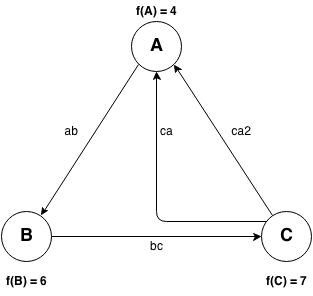
\includegraphics{lce-sample}}
\begin{description}
\item[ab] $(3,0.14,\infty,1)$,
\item[bc] $(2, 0.11, 4, 1.4)$,
\item[ca] $(2.5, 0.05, 6, 0.5)$,
\item[ca2] $(1, 0.27, \infty, 1.7)$.
\end{description}
Equilibrium equation for node $A$:
\begin{align*}
\Xi[ab]e^{0.14 (11.7 - 6)} - \Xi[ca] \Big( 1 + \frac{0.05}{6} \Big)^{ \lfloor 6 (11.7 - 4) \rfloor } - \Xi[ca2] e^{0.27 (11.7 - 4)} &= \\
\underline{2.221 \, \Xi[ab] - 1.464 \, \Xi[ca] - 7.996 \, \Xi[ca2]} &= \\
\CC_{T_G} ( 3e^{ 0.14(6 - 1), 0.14, \infty, 6 } ) &- \\
\CC_{T_G} ( 2.5 \Big( 1 + \frac{0.05}{6} \Big)^{ \lfloor 6(4 - 0.5) \rfloor }, 0.05, 6, 4 ) &- \\
 \CC_{T_G} ( e^{ 0.27 (4 - 1.7) }, 0.27, \infty, 4 ) &= \\
 \CC_{T_G} (6.041, 0.14, \infty, 6) - \CC_{T_G} ( 2.975, 0.05, 6, 4 ) - \CC_{T_G} ( 1.861, 0.27, \infty, 4 )
\end{align*}

\end{center}
\end{document}